\documentclass[11pt]{article}
\usepackage{amssymb}
\usepackage[fleqn]{amsmath}
\usepackage{hyperref}
\usepackage{graphicx}
\usepackage{semantic}

\title{Refactoring of Software Using ORM: A Formal Description}
\author{Ondrej Macek}

\begin{document}
\maketitle
\section{Introduction}
\label{sec:intro}
The evolution (change) of a software is a common issue during software development. It occurs from many reasons in all phases of software lifecycle. The evolution severity usually depends on number of changes which has to be made and on the number of affected software components. The focus of this paper is in data evolution context of software implemented in object oriented language using relational database. It means that the data evolution affect at least two software components: persistent objects (entities) and the database. The evolution is based on developer's point of view in this paper as it origins in the need to evolve code. This kind of evolution is straightforward in case there are no data stored in the database, because the database schema can be generated according to an evolved code, moreover some object-relational mapping (ORM) frameworks are able to process basic evolutionary transformation on database with stored data. The evolution of an software with ORM become more difficult when there are stored data and when the evolutionary scenario is more complex. The data migration to the new database schema is usually processed manually, which is expensive and error prone.

This paper shows how the code refactoring can be used as the source for data migration. The approach based on changes in code is useful in case when there is no model of database as it is derived directly from code. Next it can help developers to understand impact  of code changes on database. The formal description of code refactoring impact on database and stored data can help with construction of a standalone migration framework or evolutionary extension for existing ORM frameworks.

The paper is organized as follows: first the evolution of software is described in detail in Sec. \ref{sec:problem}, then the related work in presented in Sec. \ref{sec:related-work}. In Sec. \ref{sec:models} the models of software and database is provided together with a set of basic evolutionary transformations. The impact of code refactoring on database is discussed in Sec. \ref{sec:evolution}. Finally the applicability and limitations of the proposed solution is discussed in Sec. \ref{sec:contribution}.

\section{Problem Definition} 
\label{sec:problem}
A software implemented using an object-oriented language, which uses relational database as a data storage (as illustrated in the Figure \ref{fig:evolution}) is object of interest of this paper. There are three important components of such a software: application (its persistent layer concretely), database (consisting of database schema and stored data) and an ORM, therefore we define a software as a triple consisting of an application and a database which are connected together by an ORM:
\begin{align*}
& \mathbf{software} = ( Application, Database, ORM )
\end{align*}
The software has to be in consistent state so its users could have benefit from its usage. The state of the software is defined to communicate the sate of the software to its user, the symbol $\perp$ is used as a notation for inconsistent state. 
\begin{align*}
& \mathbf{state} = Consistent\; s \: | \: \perp, s \in State 
\end{align*}
The software is in consistent state if application and database are consistent and the database structure corresponds to the application structure according to the ORM.

The evolution of a software is a transformation from one consistent state to another one. These states are called generations of the software and the function which changed the state of a software are called transformations. The evolution consists of change in application and in database as shown in the Figure \ref{fig:evolution}. 
\begin{figure}
\centering
	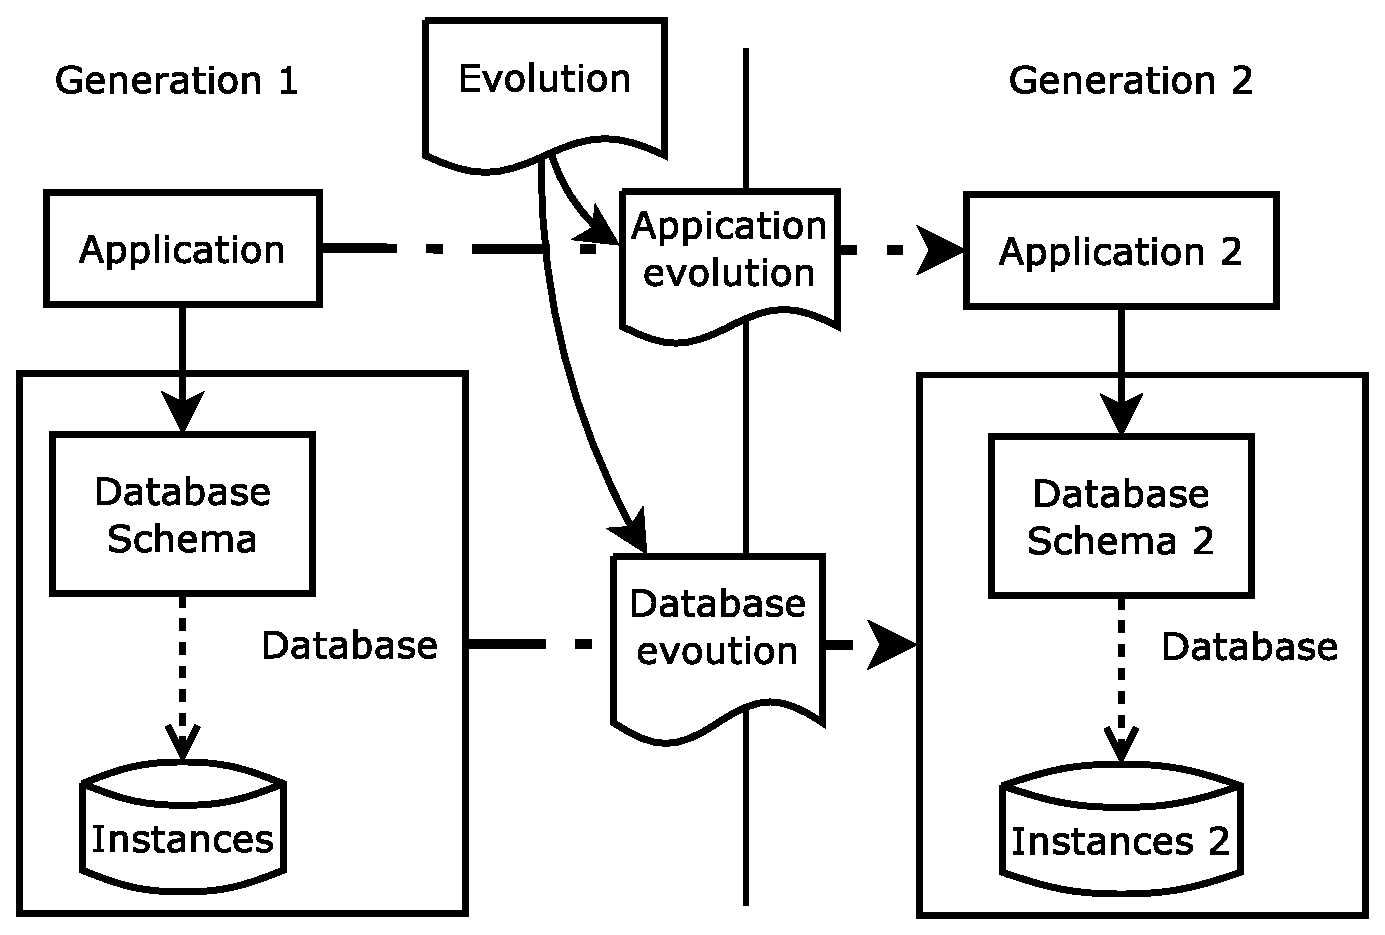
\includegraphics[scale=0.4]{./images/evolution_simple}
	\caption{The evolution of data changes the system on all levels. The figure shows all the components of the evolution process.}
	\label{fig:evolution}
\end{figure}
The usual approach is to refactor code (which is quite fast due to help of IDE) and then re-generation or manual migration of the database. Another approach is to evolve a database (e.g. due to database optimizations) and then update the code. This approach is very common too, nevertheless this paper focus on evolution which origin from the application point of view. 

The refactoring itself does not provide enough information for the complex migration of database and data, therefore a level defining the evolution is added - the set of all possible transformations $E$. The evolution definition from this level is propagated into both involved levels - application and database. The evolution is defined as:
\begin{align*}
& t(state(s)) = \begin{cases}
state(sw(\Psi(s, t), \Phi(s,t)) \; \mathbf{if} \; state(s) = Consistent \; s\\\\
 	\perp
\end{cases}\\ 
& s \in Software, t \in E
\end{align*}
Where $\Psi$ maps the software evolution cases to the code refactoring and $\Phi$ to maps to the evolutionary transformation of database.

The main issue during the software evolution is the preservation of data and information consistency. The data lost is a situation when data are damaged or lost during the migration. The information consistency means the data was transformed according to the evolution of the application and they correspond with developer's intention. 


\section{Related Work}
\label{sec:related-work}

\section{Model of Software}
\label{sec:models}
The aim of this paper is to provide an definition of data evolution, which can be applied in case of various programming language, therefore the platform independent models of application and database are introduced. These models also provide simplification, which should increase the understanding of the proposed evolutions.

\subsection{Application Model}
%TODO popis
\paragraph{Application} Application is defined as a sequence of classes and it creates the context for all structures used in the software persistent layer.
\begin{align*}
& \mathbf{Application} = (Class*)
\end{align*}

\paragraph{Class} Class represents a basic structural unit in the application model. It has a unique name, one or more properties and it can be associated to other classes in the application. 
\begin{align*}
& 	\mathbf{Class} = (label, Property*, Association*)
\end{align*}
The properties of a class can be of two kinds - values or collections - according of theirs cardinality.
	 
\paragraph{Property} Property represents a feature of a class which is represented as a primitive type. The property can be mandatory, can have a default value and according to its cardinality it can represent a single value or a collection of values. 
\begin{align*}
&	\mathbf{Property} = (label, AppType, DefaultValue, Cardinality, Mandatory)
\end{align*}

\paragraph {Association} Association represents a connection between two classes. It has a unique name and the reference is represented by the label of referenced class. The class which owns the association is consider to be the starting class of an association, referenced class is consider to be the ending class of an association. The cardinalities defines the multiplicity of both association ends.
\begin{align*}
&	\mathbf{Association} = (label, classRef, startCardinality, endCardinality) 
\end{align*}

\paragraph{Application type} Application type ($AppType$) represents primitive type in the application. There are usually defined types such as String, Integer, Boolean etc. in contrast there is only one type in our model, because we focus on structural and data changes and type casting operations are not important for us. The only $AppType$ type is called $APPSTRING$.
\begin{align*}
& \mathbf{AppType} = APPSTRING
\end{align*}

%TODO consistency

\subsection{Database Model}
he relational database consists of database schema which defines the structure of the database and data, which in our ORM system represents stored instances. The database is defined as a tuple:
\begin{align*}
&	\mathbf{Database} = ( Table*, Row* )
\end{align*}

\paragraph{Table} Table represents a basic concept of database schema. It has a unique name, one or more columns and it can be related to other tables in the schema by foreign keys. Rows in the table represents stored data.
\begin{align*}
&	\mathbf{Table} = (label, primaryKey, Column*, ForeignKey*)
\end{align*}

\paragraph{Column} Column defines data values and types which can be part of a table record.
\begin{align*}
&	\mathbf{Column} = (label, DbType, DefaultValue, Constraint*) 
\end{align*}

\paragraph{Foreign key} Foreign key is a reference to another table's primary key, it has an unique name and it can be constrained. The value of a foreign key is $\varnothing$ or a non-zero natural number.
\begin{align*}
&	\mathbf{ForeignKey} = (Label, Label, Constraint*) 
\end{align*}


\paragraph{Primary key} Primary key is unambiguous identifier of a record in a table. The primary key is always provided (automatically generated) by the database as a non-zero natural number. Primary key is always defined with constraints $NOTNULL$ and $UNIQUE$. 
\begin{align*}
&	\mathbf{PrimaryKey} =  ( Label, Sequence ) \end{align*}
The sequence generates values of primary key. The new value of a key is obtained by calling the function $next(s)$. The sequence which provides numbers incremented by one is called $s_1$ if the increment is 1, $s_{10}$ if the increment is 10 etc.

\paragraph{Data Types} Database data types $DbType$ represents primitive types in the database. There are usually defined types such as Varchar, Integer, Boolean etc. There is only one type of column values defined in the model called $DBSTRING$. Next the $DBINT$ type is defined for the values of keys.
\begin{align*}
&	\mathbf{DbType} = DBSTRING \; | \; DBINT
\end{align*}

\paragraph{Constraints} There are two types of constraints defined in the model. Both constraints are column constraints - first constraint defines non-empty columns, second constraint defines there has to be unique records in a column or foreign key.
\begin{align*}
&	\mathbf{Constraint} = NOTNULL \; | \; UNIQUE 
\end{align*}

A database consists not only from schema but also from data which are represented as rows in a table. A table row in our model is a tuple consisting of value pairs, which represents concrete value of concrete column or key. Each row contains a name of a table it belongs to.
\begin{align*}
&	\mathbf{Row} = (Label, N, Pair*) \\
&	\mathbf{Pair} = (Label, Value) 
\end{align*}

%TODO consistency

\subsection{Object Relational Mapping}
The ORM can differ from application to application, its impact on the evolution is not crucial but it has to be present to provide full information about the method. The mapping is similar to the Hibernate
mapping, thus a lot of developers should be familiar with it. 
% add mapping

\section{Data Evolution of Software}
\label{sec:evolution}
The evolution of the software is mapped to the layer specific transformation, which are defined in Sec. \ref{sec:app-evolution} and \ref{sec:db-evolution}. Finally the evolution cases and their mapping on application and database components are presented in \ref{sec:sw-evolution}. The transformations are divided into groups according to their impact on structure and data. 

%TODO evalutation of trnasformations

\subsection{Application Evolution}
\label{sec:app-evolution}
The application model defines only the structure of an application thus there are defined transformation for its creating, altering and disassembling. Therefore the conditions for successful transformations are simple 1) when creating an object in the model or altering its name collisions has to be prevent, 2) when renaming a class the references have to be updated 3) when creating or altering an association the existence of referenced class has to be verified. The only issue during disassembling is the class can be removed only in case it is not associated by other classes. If a transformation cannot be processed the state of the application become inconsistent. The transformations are in table \ref{tab:app-evolution}. The list of altering operations is not complete as there are missing transformation for changing the obligation or cardinality of properties and associations. It is because these transformations are not so important for the next text when the complex refactorings are considered. 
\begin{table}
\centering
	\begin{tabular}{|l|}
	\hline
	\textbf{Application Creation} \\
	newProperty(className, property, application) \\
	newAssociation(className, association, application) \\
	newClass(class, application) \\
	\textbf{Application Alternation} \\
	renameProperty(className, oldName, newName, application) \\
	renameAssociation(className, oldName, newName, application) \\
	renameClass(oldName, newName, application)\\
	\textbf{Application Disassembly} \\
	removeProperty(className, propertyName, application) \\
	removeAssociation(className, associationName, application) \\
	removeClass(className, application)\\
	\hline
	\end{tabular}
	\caption{The transformations for application evolution}
	\label{tab:app-evolution}
\end{table}

\subsection{Database Evolution}
\label{sec:db-evolution}



\subsection{Software Evolution}
\label{sec:sw-evolution}

\section{Contribution}
\label{sec:contribution}

\section{Conclusion}

\end{document}
